\subsection{Pre-processing}
Before extracting the planes, we performed the following pre-processing steps:

\begin{itemize}
	\item We transformed the depth component of the supplied XYZ data from the Kinect sensor into a 3D point cloud representation similar to the representation used for system 6 from the lectures, to make it easier to perform region growing to extract the planes using the lecture example code
	\item We cleaned the data by:
		\begin{itemize}
			\item removing all points from the data in which the Z co-ordinate (representing the depth of the point) was higher than a given threshold (we found that 1400 was an appropriate choice), as these were not relevant to the problem that we were trying to solve, since the only things we are interested are the cabinet and the book, which are in the foreground. and
			\item removing all points from the data in which the XYZ co-ordinates were (0,0,0), as these points were found to interfere with the plane fitting
		\end{itemize}
	\item We normalized the data by dividing all of the X,Y, and Z co-ordinate values by 5. This was found to have a favorable effect on the speed and accuracy of the region growing algorithm
\end{itemize}

Figure \ref{fig:preprocessing} illustrates the effect of our transformations. The raw XYZ depth data for frame 17 (which we used as our foundation frame) is shown in the picture on the left of the figure, and the transformed data is shown on the right. The matlab code to perform the pre-processing is shown in section \ref{planeExtractionCode} of this report.

% eliminate the background  After having observed the range data, we decided to eliminate all pixels with the range $Z > 1400$, which removed the background. Additionally we transformed the range data in X-Y space to a pointcloud which made it easier to work with and visualize (see Figure \ref{fig:foundation}).

\begin{figure}[H]
	\centering
	\begin{subfigure}[b]{0.45\textwidth}
		\centering
		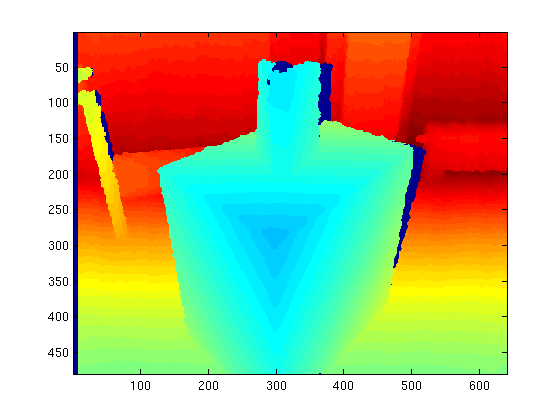
\includegraphics[width=\textwidth]{Images/1-rawZImage.png}
		\caption{}
	\end{subfigure}%
	\hspace{1cm}
	\begin{subfigure}[b]{0.45\textwidth}
		\centering
		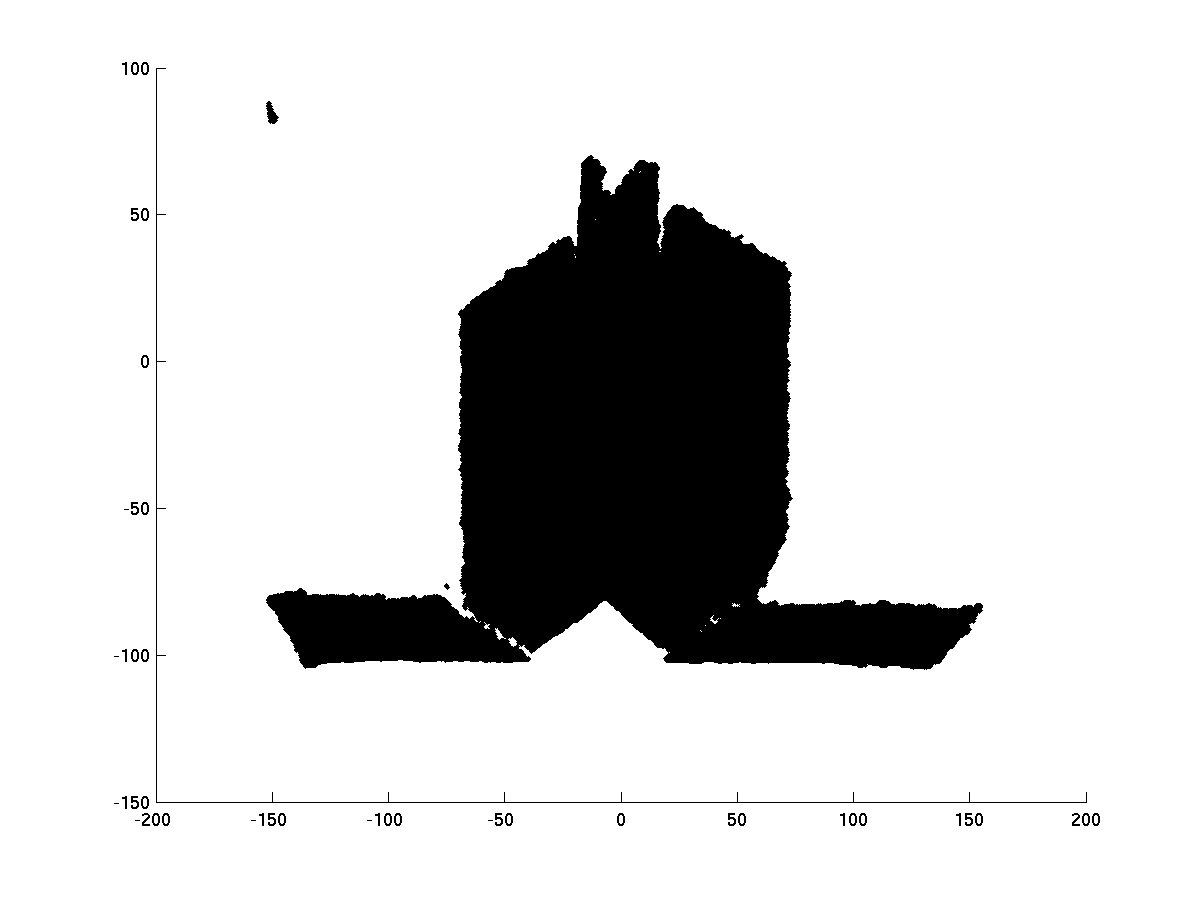
\includegraphics[width=\textwidth]{Images/3-RangeReduced.png}
		\caption{}
	\end{subfigure}
	\caption{The raw depth image from the XYZ data (a) and the same data after the pre-processing steps had been carried out (b) for our foundation frame.}
	\label{fig:preprocessing}
\end{figure}

